\section{LDU Design}

\subsection{Log-based Concurrent updates}

%Paragraph 1: Log 기반 Concurrent updates에 대한 설명
% Flat combining

% Oplog

\subsection{Approach}

%Paragraph 1: Log 기반으로 LDU에서 사용하는 방법 요약



%Paragraph 2: timestamp를 사용하지 않아도 되는 이유 설명



%Paragraph 3: CoW 기법 : read before physical update 



%Paragraph 4: 그림 설명 



\subsection{The LDU Algorithm}

%Paragraph 1:LDU 소스 코드 설명 


\subsection{logical update}
\begin{figure}[tb]
\begin{obeylines}
\begin{obeyspaces}
function \(logical\_insert(obj, root) \):
~~~If CAS(obj.del\_node.mark, 1, 0) $\ne$ 1:  
~~~    obj.add\_node.mark $\gets$ 1
~~~    If test\_and\_set\_bit(OP\_INSERT, obj.exist) $\ne$ true:
~~~        set\_bit(OP\_INSERT, obj.used):
~~~        obj.add\_node.op $\gets$ OP\_INSERT
~~~        obj.add\_node.key $\gets$ obj
~~~        obj.add\_node.root $\gets$ root
~~~        add\_lock\_less\_list(obj.add\_node)
~~~
~~~
function \(logical\_remove(obj, root) \):
~~~If CAS(obj.add\_node.mark, 1, 0) $\ne$ 1:  
~~~    obj.del\_node.mark $\gets$ 1 
~~~    If test\_and\_set\_bit(OP\_REMOVE, obj.exist) $\ne$ true:
~~~        set\_bit(OP\_REMOVE, obj.used):
~~~        obj.del\_node.op $\gets$ OP\_REMOVE
~~~        obj.del\_node.key $\gets$ obj
~~~        obj.del\_node.root $\gets$ root
~~~        add\_lock\_less\_list(obj.del\_node)

\end{obeyspaces}
\end{obeylines}
\rule{\columnwidth}{0.5pt}
\vspace{-\baselineskip}
\caption{\deferu logical update algorithm. \code{logical\_insert} represents
 non-blocking insert function.
It may be called by original insert position without locks. The fastpath is
 that when their object was removed by \code{logical\_remove},
 \code{logical\_insert} just changes node's marking field.}
\label{fig:logicalupdate}
\end{figure}


\subsection{Physical update}
\begin{figure}[tb]
\begin{obeylines}
\begin{obeyspaces}
function \(synchronize\_ldu(obj, head) \):
~~~If (head.first = NULL): 
~~~    return; 
~~~entry $\gets$ xchg(head.first, NULL);
~~~for each list node:
~~~    obj $\gets$ node.key
~~~    clear\_bit(node.op, obj.exist)
~~~    If !xchg(node.mark, 0):
~~~         physical\_update(node.op, obj, node.root)
~~~    clear\_bit(node.op, obj.used)
~~~
function \(physical\_update(op, obj, root) \):
~~~If op = OP\_INSERT :  
~~~    call real insert function(obj, root) 
~~~Else If op = OP\_REMOVE :  
~~~    call real remove function(obj, root) 

\end{obeyspaces}
\end{obeylines}
\rule{\columnwidth}{0.5pt}
\vspace{-\baselineskip}
\caption{\deferu physical update algorithm. \code{synchronize\_ldu} may be
 called by reader and converts update log to original data structure
 traversing the lock-less list.}
\label{fig:physicalupdate}
\end{figure}




%$$$$$$$$$$$$$$$$$$$$$$$$$$$$$$$$$$$$$$$$$$$$$$$$$$$$$$$$$$$$$$$$$$$$$$$$$$$$$$$$
%Reference Sentence 1
%$$$$$$$$$$$$$$$$$$$$$$$$$$$$$$$$$$$$$$$$$$$$$$$$$$$$$$$$$$$$$$$$$$$$$$$$$$$$$$$$

%To keep the log from growing without end, we can at any point apply in-order a
%subsequence of the operations at the head of the log to the state to derive a
%new state, and remove these operation from the log[EuroSys 2006 PLS].

%High level operations performed on shared data structures can be divided into
%three groups: read-only, write-only, and read-modify-write[PLS].

%Read-only operations do not mutate the data, write-only operations modify the
%data but do not return a result, and read-modify-write operations change shared
%data and return a result that is dependent on the data read[PLS].

%Both suffer from a complete loss of scalability beyond a rather low concurrency
%level, because all threads must succesfully apply a CAS operation to the shared
%head or tail of the queue in order to complete their operation[FC].


%$$$$$$$$$$$$$$$$$$$$$$$$$$$$$$$$$$$$$$$$$$$$$$$$$$$$$$$$$$$$$$$$$$$$$$$$$$$$$$$$
%Reference Sentence 2
%$$$$$$$$$$$$$$$$$$$$$$$$$$$$$$$$$$$$$$$$$$$$$$$$$$$$$$$$$$$$$$$$$$$$$$$$$$$$$$$$

%This section describes the \deferu algorithm, a lightweight concurrent
%update for update-heavy data structures based on deferred updates.
%Challenges to designing a deferred update mechanism includes 
%performing concurrent update with minimal
%cache line transfers allowing parallel updates.
%At each update operation, \deferu records this update
%operation log to lock-less list.
%Before the read operation, \deferu applies the updates log in chronological
%order.
%In order to deferred update, \deferu divide the update operation 
%into \emph{logical update} and
%\emph{physical update}.
%The \emph{logical update} inserts logs into the lock-less list and carries out
%update side absorbing; on the other hand, the \emph{physical update} executes
%these operations that are minimized by the update side absorbing.

%\begin{figure}[tb]
%  \begin{center}
    %
    % 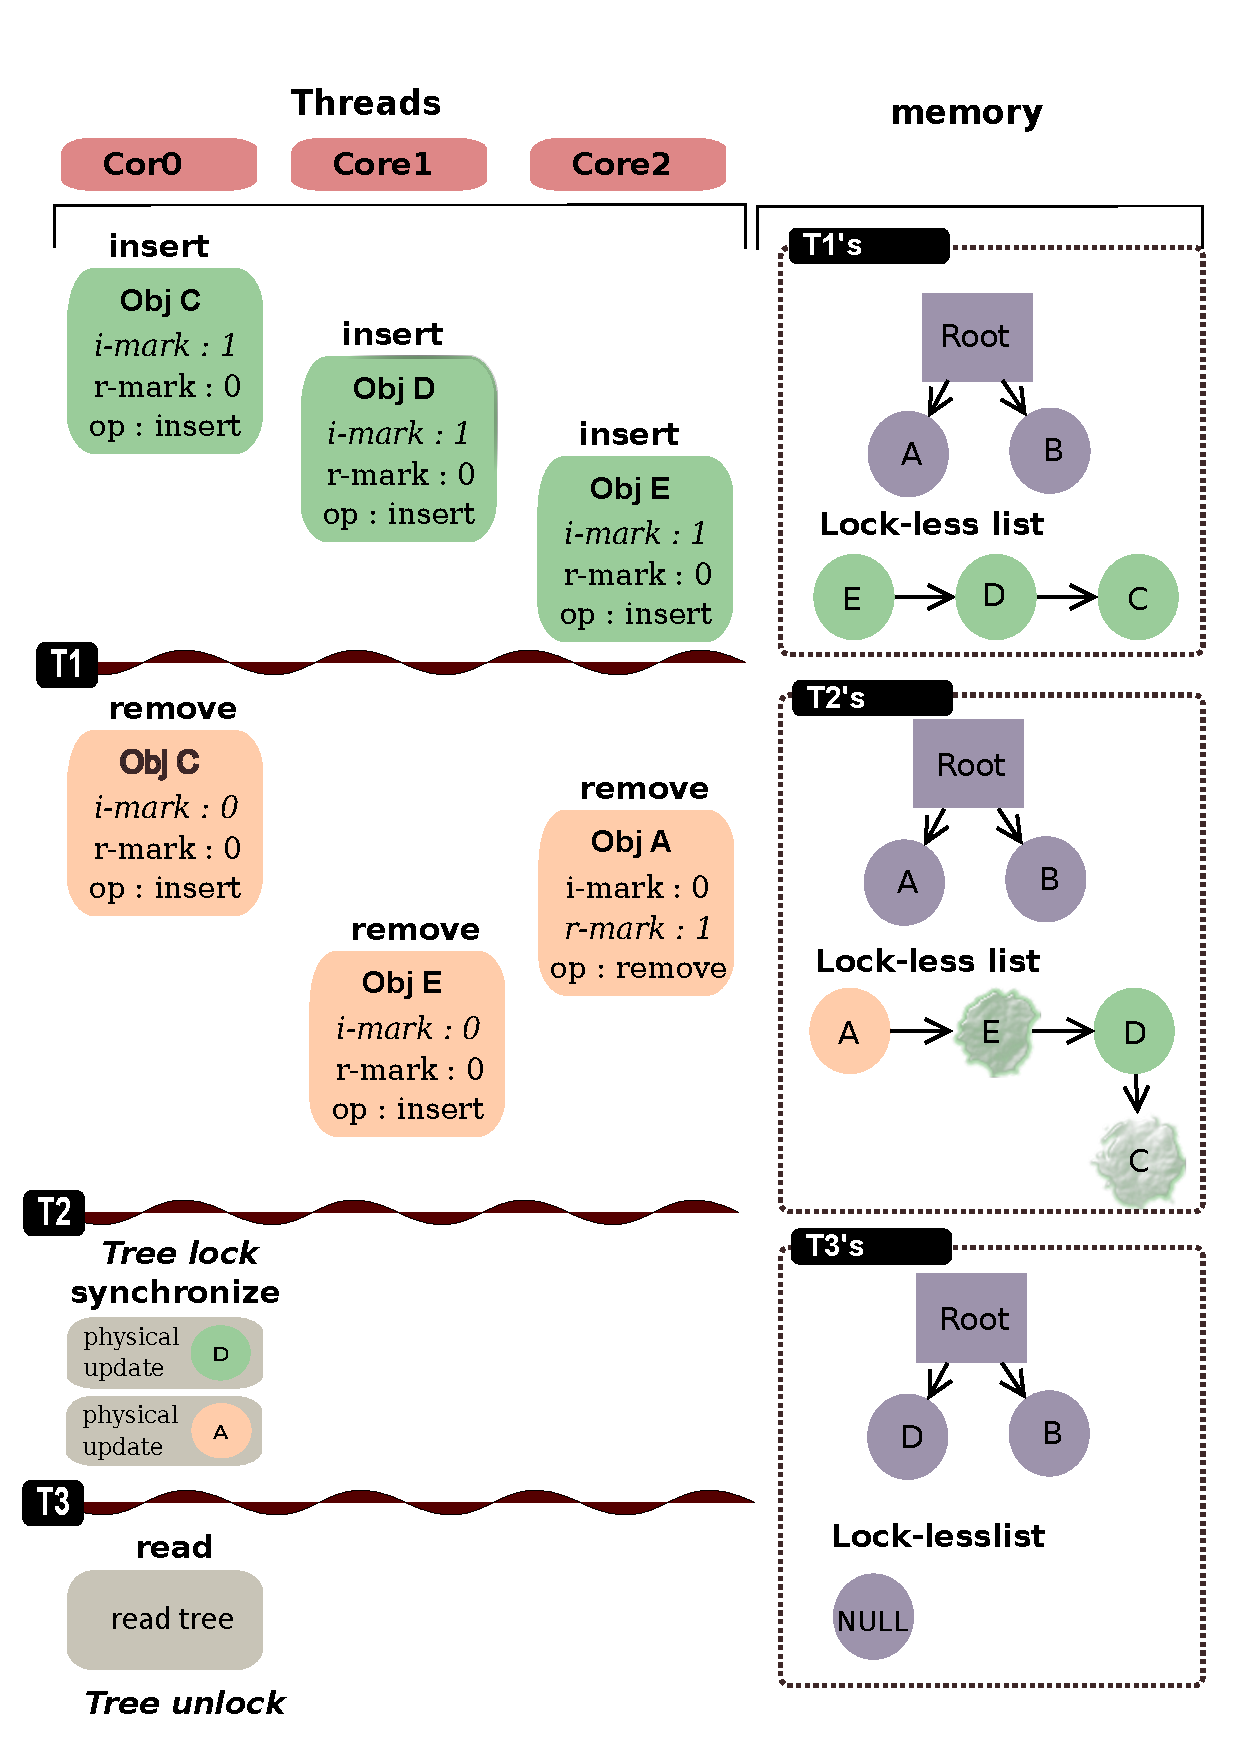
\includegraphics[width=0.5\textwidth,height=0.5\textheight,keepaspectratio]{fig/basic}
%  \end{center}
%  \caption{\deferu example showing six update operations and one read
%  operation. The execution flows from top to bottom. Memory represents original
%  data structure and logging queue at T1, T2 and T3, respectively.}
%  \label{fig:basic}
%\end{figure}

%\subsection{Approach}

%\deferu's scheme for concurrent update is proposed to overcome limitations
%of Linux kernel where 
%both insert and remove operations must not be invoked concurrently for the same
% object, but reads can be concurrently invoked with update.
%\deferu borrows ideas from Oplog's deferred processing and Harris' marking
% scheme.
%The reason is that Linux kernel's object management scheme differs from
% research-oriented data structure such as the lock-free and wait-free data
% structures~\cite{Harris2001Lockfree}~\cite{Fomitchev2004Lockfree}~\cite{Timnat2012}.
%For example, consider the Harris linked list, an insert operation inserts an 
%integer key into the data structure, but Linux kernel inserts their object link.
%The Linux kernel's list operations do not depend on key value.
%Furthermore, Harris linked list node's constructor can be invoked
%upon the insert function's scope, but Linux kernel's node is created on outside scope.
%In this regard, if duplicated remove operation occur, the Linux kernel may
%fail because their link pointer had been freed from destructor.
%Therefore, if a operation is an insert operation, the after operation must occurs 
%remove operation with regard to same object;the remove must execute after the 
%insert, or insert must execute after the remove.
%It means that updates such as insert and remove must not concurrently occur at
%the same object, but reads can occur concurrently.
%\deferu scheme inspires by this operation sequence, and inherits ideas
%from Oplog's deferred processing and Harris's marking scheme.

%\deferu's scheme for concurrent update inspires by Linux kernel's operation
%sequence.
%For example, consider a linked list in Linux kernel, if a operation is an insert
%operation, the after operation must occurs remove operation because Linux
%kernel's object management scheme differs from research-oriented data structure
%such as the lock-free and wait-free data
%structures~\cite{Harris2001Lockfree}~\cite{Fomitchev2004Lockfree}.
%Linux kernel's list operations do not depend on key value, but their 
%list operations depend on their object.
%These structure are their node's constructor can be invoked upon the insert
%function's scope, but Linux kernel's node is created on outside scope.
%In this regard, if duplicated remove operation occur, the Linux kernel may
%fail because their link pointer had been freed from destructor.
%Therefore, the remove must execute after the insert, or insert must execute
%after the remove.
%It means that updates such as insert and remove cannot concurrently occur at
%the same object, but reads can occur concurrently.
%\deferu scheme inspires by this operation sequence, and inherits ideas
%from Oplog's deferred processing and Harris's marking scheme.

%One important algorithm in our proposed novel concurrent update scheme is
%update-side absorbing operation that cancels duplicated operations for
% optimizations.
%A new remove operation, for example, may cancel an existing insert operation
%with regard to same object, so reader can eventually reads consistent data.
%Even though the Oplog's absorbing operation is invoked by
%read, \deferu's absorbing operation is fully invoked by update, so read-side
%performance is enhanced.

%The basic principle of update-side absorbing is that update uses atomic 
%marking operation for the object's mark field, which allows previous operation
% to cancel.
%For instance, if a new remove operation occurs after insert operation of the
%same object, \deferu does not store this operation in the lock-less
%list; instead, it changes the insert mark field to zero using the CAS.
%This mark is checked later when reading operation occurs and the operation log 
%maintained in the lock-less list is applied to original data structure
% atomically.
%This action may give effective update;however, the inserted operation log has
% remained in the lock-less list, so \deferu's reader checks the mark field
% when they convert operation log to original data structure atomically.

%figure : basic principle 
%Figure \ref{fig:basic} gives an example of deferred update with six update
%operations and one read operation.
%In this figure, execution flows from top to bottom.
%The data structure for \emph{physical update} is a tree, and initial values in
%the tree are node \code{A} and \code{B}.
%In contrast, the data structure for \emph{logical update} is lock-less list.
%In the top figure, \code{Core0}, \code{Core1} and \code{Core2} perform the
%logical insert operation to nodes \code{C}, \code{D} and \code{E},
% respectively.
%The logical inserts set the insert mark, and they then insert their
%nodes into lock-less list.
%In this case, none of the lock is needed because \deferu uses the lock-less
%list;all threads can execute the update concurrently.
%At \code{T1}, the tree contains node \code{A}
%and \code{B} and 
%the lock-less list contains node \code{E}, \code{D} and \code{C}.
%When removing the node \code{C}, the node \code{C}, whose mark field was marked
%by insert, atomically cleans up the insert marked field.
%At \code{T2}, the lock-less list contains nodes
%\code{A}, \code{E}, \code{D}, and \code{C}, and the marking field is zero for 
%nodes \code{E} and \code{C}.
%Before running the \code{synchronize} function, they need to lock the original
% tree's lock using the exclusive lock in order to protect the tree's
% operation.
%The \code{synchronize} migrates from lock-less list node to tree node, each of 
%which is the marked node, so nodes \code{A} and \code{D} are migrated.
%Finally, the tree contains nodes \code{D} and \code{B}, so the reader can read
% eventually consistent data.

%First, removing the cancelable operation at update point, \deferu uses the
% update side absorbing instead of read before absorbing.
%Therefore, read before operations in \deferu are fast because read-side
%absorbing operation is eliminated. 
%One notable difference between Oplog and \deferu is that 
%\deferu uses a light weight global queue with non-blocking synchronization 
%for update logs and eliminates time stamps while Oplog is dependent on 
%per-core logs with time stamps.
%By eliminating the global time stamps(hardware-dependent feature), \deferu is
% not dependent on hardware feature.
%Furthermore, update operations in \deferu are also fast because they use
%efficient update-side absorbing that eliminates traversal finding the
%cancelable operation.
%Furthermore, to optimize the log management and minimize the traversal
% overheads during reading, \deferu applies efficient update-side absorbing
% algorithm instead of read-side absorbing algorithm.

%\subsection{logical update}
%\begin{figure}[tb]
%\begin{obeylines}
%\begin{obeyspaces}
%function \(logical\_insert(obj, root) \):
%~~~If CAS(obj.del\_node.mark, 1, 0) $\ne$ 1:  
%~~~    obj.add\_node.mark $\gets$ 1
%~~~    If test\_and\_set\_bit(OP\_INSERT, obj.exist) $\ne$ true:
%~~~        set\_bit(OP\_INSERT, obj.used):
%~~~        obj.add\_node.op $\gets$ OP\_INSERT
%~~~        obj.add\_node.key $\gets$ obj
%~~~        obj.add\_node.root $\gets$ root
%~~~        add\_lock\_less\_list(obj.add\_node)
%~~~
%~~~
%function \(logical\_remove(obj, root) \):
%~~~If CAS(obj.add\_node.mark, 1, 0) $\ne$ 1:  
%~~~    obj.del\_node.mark $\gets$ 1 
%~~~    If test\_and\_set\_bit(OP\_REMOVE, obj.exist) $\ne$ true:
%~~~        set\_bit(OP\_REMOVE, obj.used):
%~~~        obj.del\_node.op $\gets$ OP\_REMOVE
%~~~        obj.del\_node.key $\gets$ obj
%~~~        obj.del\_node.root $\gets$ root
%~~~        add\_lock\_less\_list(obj.del\_node)

%\end{obeyspaces}
%\end{obeylines}
%\rule{\columnwidth}{0.5pt}
%\vspace{-\baselineskip}
%\caption{\deferu logical update algorithm. \code{logical\_insert} represents
% non-blocking insert function.
%It may be called by original insert position without locks. The fastpath is
% that when their object was removed by \code{logical\_remove},
% \code{logical\_insert} just changes node's marking field.}
%\label{fig:logicalupdate}
%\end{figure}

%The pseudo code for \deferu's \emph{logical update} is given in
%figure~\ref{fig:logicalupdate}.
%The \code{logical\_insert}, the concurrent update function, checks whether this
%object already has been removed by \code{logical\_remove}.
%If this object has been removed, \code{logical\_insert} initializes the marking
% field and then they return, which is fastpath.
%The marking field needs synchronization because this field in the
%\emph{logical update} is shared with the \emph{physical update}, so the CAS
% operation is needed.
%When the marking field has been initialized, they set the
%marking field, then they check whether or not this node already has been
% inserted in lock-less list.
%If the node does not exist in lock-less list, then they insert the node into
%lock-less list.

%\subsection{Physical update}
%\begin{figure}[tb]
%\begin{obeylines}
%\begin{obeyspaces}
%function \(synchronize\_ldu(obj, head) \):
%~~~If (head.first = NULL): 
%~~~    return; 
%~~~entry $\gets$ xchg(head.first, NULL);
%~~~for each list node:
%~~~    obj $\gets$ node.key
%~~~    clear\_bit(node.op, obj.exist)
%~~~    If CAS(node.mark, 1, 0) = 1:
%~~~         physical\_update(node.op, obj, node.root)
%~~~    clear\_bit(node.op, obj.used)
%~~~
%function \(physical\_update(op, obj, root) \):
%~~~If op = OP\_INSERT :  
%~~~    call real insert function(obj, root) 
%~~~Else If op = OP\_REMOVE :  
%~~~    call real remove function(obj, root) 

%\end{obeyspaces}
%\end{obeylines}
%\rule{\columnwidth}{0.5pt}
%\vspace{-\baselineskip}
%\caption{\deferu physical update algorithm. \code{synchronize\_ldu} may be
% called by reader and converts update log to original data structure
% traversing the lock-less list.}
%\label{fig:physicalupdate}
%\end{figure}

%The pseudo code for \deferu's \emph{physical update} is given in
%Figure~\ref{fig:physicalupdate}.
%First, they check whether lock-less list is an empty list or not, then they
%iterate the lock-less list.
%If the marking field has been set, they execute migration from
%lock-less to original data structure.
%Because the marking field in \emph{physical update} is shared with
% \emph{logical update}, the CAS operation is needed.
%They initialize the used field, which needs to protect the object from freed
% through destructor.
%The programmer must acquire locks on the \code{synchronize\_ldu} function,
%which migrates log to original data structure.
%Finally, the \code{physical\_update} executes original functions by using the
%operation log.
